\subsection{Low Energy \piz Production}\label{sec:into:xsection.low}

\begin{figure}[h!]\begin{center}
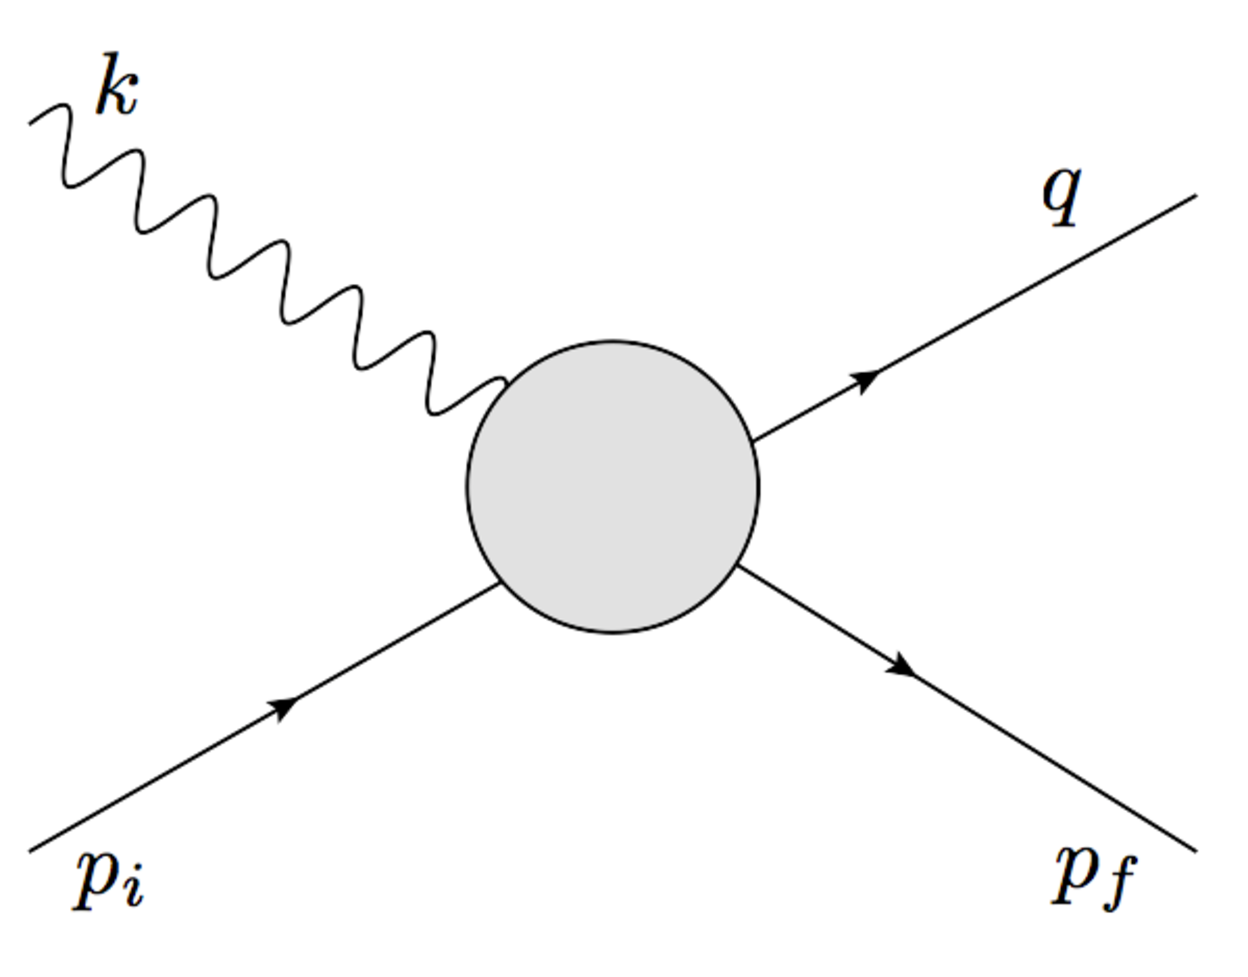
\includegraphics[width=0.5 \figwidth,height= \qfigheight]{\figures/feyman_pi0IV.pdf}
\caption[Diagram for \piz Photoproduction]{\label{fig:xsection.pi0feynman}	Diagram for photoproduction of the \piz meson. $k$ and $p_i$ are the incident photon beam and target proton 4-moment respectively, $q$ and $p_f$ represent the produced \piz meson and scattered proton 4-momenta respectively.}
\end{center}\end{figure}
For incoming photon beam energies less than 2.8~GeV, the production of the \piz meson, with 4-momenta $q$, in photon-proton reactions, with 4-momenta $k$ and $p_i$ respectively and $p_f$ being the 4-momenta of the scattered proton (see Fig.~\ref{fig:xsection.pi0feynman}),  can be described in terms of the three Lorentz invariant Mandelstam variables, $s$, $t$ and $u$, where
\begin{align}
s = (k+p_i)^2 = (q+p_f)^2 \nonumber \\
t=(p_i-p_f)^2 = (k-q)^2  \nonumber \\
u = (k - p_f)^2 = (p_i-q)^2 \ .
\end{align}
The sum of the Mandelstam variables linearly combine to give the sum of masses of the particles involved:
\begin{align}
s + t + u = \sum\limits_{i}^{4} m_i^2 
\end{align}
and the definition of Lorentz-invariant mass:
\begin{align}
p_i\cdot p_i = E_i^2 - \mathbf{p_i}\cdot \mathbf{p_i} = m_i^2 \ .
\end{align}
Using energy-momentum conservation:
\begin{align}
k + p_i = q+p_f \,
\end{align}
it is seen that only three of the four momenta are independent. Conventionally the use of $k$ and $q$ and a combined 4-momenta of the nuclei 
\begin{align}
P = \frac{1}{2}(p_i+p_f)
\end{align}
are used as the independent kinematic variables. The three Mandelstam variables can be express in terms of the other two, therefore the scattering process is described by functions of only two other the Mandelstam variables. Conventionally they are chosen to be $s$ and $t$, which in the center-of-mass frame (C.M.) of the initial and final state equal the invariant mass squared of the system and the momentum transfer in the production process respectively.
The scattering matrix $\mathcal{M}$ for single pion photoproduction process is written as:
\begin{align}
\mathcal{M} =  (\epsilon_\mu k_\nu - \epsilon_\nu k_\mu)&[ \frac{1}{2}i \gamma_5 \gamma_\mu \gamma_\nu A_1(s,t) + 2 i \gamma_5 P_\mu(q-\frac{1}{2}k)_\nu A_2(s,t) \nonumber \\ & + \gamma_5 \gamma_\mu q_\nu A_3(s,t) + \gamma_5 \gamma_\mu(2P_\nu- i M\gamma_\nu) A_4(s,t) ] \ ,
\end{align}
where $M$ is the nucleon mass, $\epsilon$ is the photon polarization and $A_i(s,t)$ are the invariant functions of the Mandelstam invariants $s$ and $t$. To obtain the scattering matrix elements in terms of experimental quantities, it is preferred and easier to work in the C.M. system and reduce the $\mathcal{M}$ to a form $\mathcal{F}$ by equating the invariant form of the scattering matrix elements in each frame, i.e.:
\begin{align}
\bar{u}(p_2)\mathcal{M} u(p_1) \equiv \frac{4 \pi W}{M}\chi_f^\dagger \mathcal{F} \chi_i \ ,
\end{align}
where $\bar{u}(p_2)$ and $u(p_1)$ are final and initial state Dirac spinors respectively and $\chi_f$ and $\chi_i$ are final and initial state Pauli spinors. The differential cross-section for single pion production is:
\begin{align}
\frac{d\sigma}{d\Omega} = \frac{q}{k}| \bra{f}\mathcal F \ket{i}|^2,
\end{align}
The expression to express Dirac spinors in terms of Pauli spinors is written as:
\begin{align}
\mathcal{F} = & i\vec{\mathbf{\sigma}}\cdot \vec{\mathbf{\epsilon}} \mathcal{F}_1 + \frac{1}{qk}(\vec{\mathbf{\sigma}}\cdot \vec{\mathbf{q}})\vec{\mathbf{\sigma}} \cdot(\vec{\mathbf{k}}\times \vec{\mathbf{\epsilon}}) \mathcal{F}_2 \nonumber \\ & + \frac{i}{qk}(\vec{\mathbf{\sigma}}\cdot \vec{\mathbf{k}})(\vec{\mathbf{q}}\cdot \vec{\mathbf{\epsilon}})\mathcal{F}_3 + \frac{i}{q^2}(\vec{\mathbf{\sigma}}\cdot \vec{\mathbf{q}})(\vec{\mathbf{q}}\cdot \vec{\mathbf{\epsilon}})\mathcal{F}_4 \ ,
\end{align}
where $\vec{\mathbf{k}}$ and $\vec{\mathbf{q}}$ are the C.M. 3-momenta and $\vec{\mathbf{\epsilon}}$ is the polarization of the photon. The relationship between $A_i$ and $\mathcal{F}$ is found using the relations:
\begin{align}
\mathcal{F}_1 = \frac{W- M}{8 \pi W }(D_1 D_2)^{\frac{1}{2}}\left[ A_1+(W-M)A_4 - \frac{k_0q_0-\vec{\mathbf{k}}\cdot \vec{\mathbf{q}}}{W-M}(A_3-A_4)\right] \\
\mathcal{F}_2 = qk \frac{W- M}{8 \pi W }(\frac{D_2}{D_1})^{\frac{1}{2}}\left[ -A_1+(W+M)A_4 + \frac{k_0q_0-\vec{\mathbf{k}}\cdot \vec{\mathbf{q}}}{W+M}(A_3-A_4)\right]  \\
\mathcal{F}_3 =qk \frac{W- M}{8 \pi W }(D_1 D_2)^{\frac{1}{2}}q\left[(W-M)A_2 + A_3 - A_4\right]\\
\mathcal{F}_4 = q^2 \frac{W- M}{8 \pi W }(\frac{D_2}{D_1})^{\frac{1}{2}}q\left[ -(W+M)A_2 + A_3 - A_4\right] 
\end{align}
where
\begin{align}
D_1 = (M^2 + \vec{\mathbf{k}}^2)^{\frac{1}{2}}+M \\
D_2 = (M^2 + \vec{\mathbf{q}}^2)^{\frac{1}{2}}+M \ .
\end{align}
$\mathcal{F}_i(s,t)$ are known as structure functions, alternatively known by Chew, Goldberger, Low and Nambu (\abbr{CGLN}) amplitudes. These amplitudes describe photoproduction as a function of $s$ and $t$, and therefore in terms of momentum transfer. To represent the process in terms of angular momentum transitions, expansion of the structure functions as partial waves in derivatives of Legendre polynomials, $P_l^\prime(\cos\theta)$, results in the four multipole series:
\begin{align}
&&\mathcal F_1 = \displaystyle\sum_{l=0}^{\infty}[lM_{l+} + E_{l^+}]P_{l+1}^{\prime}(\cos\theta) + [(l+1)M_{l-1} + E_{l-}]P_{l-1}^{\prime}(\cos\theta)\\
&&\mathcal F_2 = \displaystyle\sum_{l=1}^{\infty}[(l+1)M_{l+}+lM_{l-}]P_{l}^{\prime}(\cos\theta)\\
&&\mathcal F_3 = \displaystyle\sum_{l=1}^{\infty}[E_{l+}-M_{l+}]P_{l+1}^{\prime \prime}(\cos\theta) + [E_{l-} + M_{l-}]P_{l-1}^{\prime \prime}(\cos\theta)\\
&&\mathcal F_4 = \displaystyle\sum_{l=1}^{\infty}[M_{l+} - E_{l+} - M_{l-} - E_{l-}]P_{l}^{\prime \prime}(\cos\theta)
\end{align}
The energy-dependent amplitudes $M_{l\pm}$ and $E_{l\pm}$ refer to transitions initiated by magnetic and electric radiation, respectively, leading to final states of orbital angular momentum $l$ and total angular momentum $j=l\pm\frac{1}{2}$. 


 by the formalism presented in~\cite{ar90}. The helicity amplitudes can be reconstructed by electric $(E_{l\pm})$ and magnetic $(M_{l\pm})$ multipole amplitudes of the \piz wave, where $l$ is angular momentum of the final state with total angular momentum $ j=l\pm \frac{1}{2}$. The helicity amplitudes can be written as; 
%
\begin{align}
H_{N}(\theta) = \sqrt{\frac{1}{2}}\cos\frac{1}{2}\theta \sum_{l=0}^{\infty} {[ (l+2)E_{l+} + lM_{l+} + lE_{(l+1)-} - (l+2)M_{(l+1)-}]( P^{\prime}_{l}-P^{\prime}_{l+1})}  \nonumber \ , \\
%
H_{SP}(\theta) = \sqrt{\frac{1}{2}}\cos\frac{1}{2}\theta \sin \theta \sum_{l=1}^{\infty} {[ E_{l+} - M_{l+} - E_{(l+1)-} - M_{(l+1)-}]( P^{\prime \prime}_{l}-P^{\prime \prime}_{l+1})} \ , \nonumber \\
%
H_{SA}(\theta) = \sqrt{\frac{1}{2}}\sin\frac{1}{2}\theta \sum_{l=0}^{\infty} { [(l+2)E_{l+} + lM_{l+} - lE_{(l+1)-} + (l+2)M_{(l+1)-}]( P^{\prime}_{l}+P^{\prime}_{l+1})} \ ,\nonumber \\
%
H_{D}(\theta) = \sqrt{\frac{1}{2}}\sin\frac{1}{2}\theta \sin \theta \sum_{l=1}^{\infty} {[ E_{l+} - M_{l+} + E_{(l+1)-} + M_{(l+1)-}]( P^{\prime \prime}_{l}+P^{\prime \prime}_{l+1})} \ , 
\end{align}
%
where the subscript $N$ means non-spin-flip; $D$, double spin-flip; $SP$, spin-flip with photon and 
initial nucleon having parallel spins; and $SA$, spin-flip with photon and initial nucleon having 
anti-parallel spins, $P^{\prime}$ and $P^{\prime \prime}$ are associated Legendre functions of
first and second order respectively.
%
The \piz in the photon-proton reaction channel can be described in terms of isospin amplitudes:
%
\begin{align}
	H^{\pi^0p} =& (H^{1/2} + \frac{2}{3}H^{3/2}),&\nonumber
\end{align}
The superscripts $\frac{1}{2}$ and $\frac{3}{2}$ refer to the isospin. In terms of bilinear combinations of the helicity amplitudes the observables are represented as follows:
\begin{align}
	\sigma(\theta) = \frac{q}{2k}[|H_{N}(\theta)|^2 + |H_{D}(\theta)|^2 + |H_{SP}(\theta)|^2 + |H_{SA}(\theta)|^2],\nonumber\\
	P(\theta)\sigma(\theta) = -\frac{q}{k}Im[H_{SP}(\theta)H_{D}^*(\theta) + H_{N}(\theta)H^*_{SA}(\theta)],\nonumber\\
	\Sigma(\theta)\sigma(\theta) = \frac{q}{k}Re[H_{SP}(\theta)H_{SA}^*(\theta) - H_{N}(\theta)H^*_{D}(\theta)],\nonumber\\
	T(\theta)\sigma(\theta) = \frac{q}{k}Im[H_{SP}(\theta)H_{N}^*(\theta) + H_{D}(\theta)H^*_{SA}(\theta)],\nonumber\\
	G(\theta)\sigma(\theta) = -\frac{q}{k}Im[H_{SP}(\theta)H_{SA}^*(\theta) + H_{N}(\theta)H^*_{D}(\theta)],\nonumber\\
	H(\theta)\sigma(\theta) = -\frac{q}{k}Im[H_{SP}(\theta)H_{D}^*(\theta) + H_{SA}(\theta)H^*_{N}(\theta)].
\end{align}
Here $\sigma$ is the total cross-section and $P,\Sigma$, and $T$ are the asymmetries arising from polarized recoil nucleons, polarized incident photons, and polarized target, respectively. The $G$ and $H$ observables involve both polarized photons and polarized target. The variables $q$ and $k$ refer, respectively, to the center-of-mass frame momenta of the pions and the photon.
%
\subsubsection{Helicity Partial-Wave Amplitudes}\label{sec:into:helicity}
%
Instead of using electric and magnetic multipole amplitudes as basic elements one can use helicity partial-wave amplitudes $A_{l\pm}$ and $B_{l\pm}$, which are related to the multipoles through the relations
%
\begin{align}
A_{l\pm} = \frac{1}{2}[(l+2)E_{l+} + lM_{l+}],\nonumber\\
B_{l+} = E_{l+} - M_{l+},\nonumber\\
A_{(l+1)-} =  \frac{1}{2}[(l+2)M_{(l+1)-}-lE_{(l+1)-}],\nonumber\\
B_{(l+1)-} = E_{(l+1)-} + M_{(l+1)-}.
\end{align}
%
Relation between helicity amplitudes and partial-wave amplitudes $A_{l\pm}$ and $B_{l\pm}$ can then be presented as follows
%
\begin{align}
H_{N}(\theta) = \sqrt{2}\cos\frac{1}{2}\theta \displaystyle\sum_{l=0}^{\infty} {(A_{l+} - A_{(l+1)-} )( P^{\prime}_{l}-P^{\prime}_{l+1})} \ ,\nonumber\\
%
H_{SP}(\theta) = \sqrt{\frac{1}{2}}\cos\frac{1}{2}\theta \sin \theta \displaystyle\sum_{l=1}^{\infty} {( B_{l+} - B_{(l+1)-} )( P^{\prime \prime}_{l}-P^{\prime \prime}_{l+1})} \ ,\nonumber \\
%
H_{SA}(\theta) = \sqrt{2}\sin\frac{1}{2}\theta \displaystyle\sum_{l=0}^{\infty} { (A_{l+}  + A_{(l+1)-})( P^{\prime}_{l}+P^{\prime}_{l+1})} \ ,\nonumber\\
%
H_{D}(\theta) = \sqrt{\frac{1}{2}}\sin\frac{1}{2}\theta \sin \theta \sum_{l=1}^{\infty} {( B_{l+} + B_{(l+1)-})( P^{\prime \prime}_{l}+P^{\prime \prime}_{l+1})}.
\end{align}
%
These amplitudes are related to those of Walker ~\protect\cite{Walker}, $H_1,...,H_4$, as
%
\begin{align}
H_1\equiv H_{SP}, \qquad H_2\equiv H_{N}, \qquad H_3\equiv H_D, \qquad H_4\equiv H_{SA}
\end{align}
%
Consequently $\pi^{\circ}$ photoproduction  cross section takes the following form
%
\begin{align}
	\sigma(\theta) = \frac{q}{2k}[|H_{1}(\theta)|^2 + |H_{2}(\theta)|^2 + |H_{3}(\theta)|^2 + |H_{4}(\theta)|^2]
\end{align}
%
\subsubsection{CGLN Amplitudes}
%
The CGLN ~\protect\cite{CGLN} derived the pion photoproduction cross section in terms of the  amplitudes $\mathcal F$ 
%
\begin{align}
\frac{d\sigma}{d\Omega} = \frac{q}{k}|<2|\mathcal F|1>|^2,
\end{align}
where $q$ and $k$ are three momenta of the pion and photon in center-of-mass frame, respectively.
%
For a given isotopic spin configuration, the amplitude $\mathcal F$ is written in terms of the following combinations of Pauli-spin matrices
%
\begin{align}
\mathcal {F} = i\bf \sigma \cdot \bf \epsilon \mathcal F_1 + \frac{\bf \sigma\cdot  q\sigma \cdot (k \times\bf  \epsilon)}{qk}\mathcal F_2+
\frac{i\bf \sigma\cdot \bf k\bf q\cdot \bf \epsilon}{qk}\mathcal F_3 + \frac{i\bf \sigma \cdot \bf q \bf q \cdot \bf \epsilon}{q^2} \mathcal F_4
\end{align}
where $\sigma$'s are Pauli-spin matrices and $\epsilon$ is a photon helicity.
%
In terms of electric and magnetic multipoles the functions $\mathcal F_1...\mathcal F_4$ take an explicit form through an expansion involving derivatives of Legendre polynimials:
%
\begin{align}
&&\mathcal F_1 = \displaystyle\sum_{l=0}^{\infty}[lM_{l+} + E_{l^+}]P_{l+1}^{\prime} + [(l+1)M_{l-1} + E_{l-}]P_{l-1}^{\prime}\\
&&\mathcal F_2 = \displaystyle\sum_{l=1}^{\infty}[(l+1)M_{l+}+lM_{l-}]P_{l}^{\prime}\\
&&\mathcal F_3 = \displaystyle\sum_{l=1}^{\infty}[E_{l+}-M_{l+}]P_{l+1}^{\prime \prime} + [E_{l-} + M_{l-}]P_{l-1}^{\prime \prime}\\
&&\mathcal F_4 = \displaystyle\sum_{l=1}^{\infty}[M_{l+} - E_{l+} - M_{l-} - E_{l-}]P_{l}^{\prime \prime}
\end{align}
%
The obtained relations between helicity amplitudes of Walker~\protect\cite{Walker} in terms of CGNL  $\mathcal F's$ \\are presented as following:
%
\begin{align}
&&H_1(\theta,\phi) = -(1/\sqrt{2})e^{i\phi}sin\theta\cos\frac{1}{2}\theta (\mathcal F_3 + \mathcal F_4),\\
&&H_2(\theta,\phi) = \sqrt{2}\cos\frac{1}{2}\theta [(\mathcal F_2 - \mathcal F_1) + \frac{1}{2}(1 - \cos\theta)(\mathcal F_3 - \mathcal F_4)],\\
&&H_3(\theta,\phi) = (1/\sqrt{2})e^{2i\phi}\sin\theta\sin\frac{1}{2}\theta(\mathcal F_3 - \mathcal F_4),\\
&&H_4(\theta,\phi) = \sqrt{2}e^{i\phi} \sin \frac{1}{2}\theta[(\mathcal F_1 + \mathcal F_2) + \frac{1}{2}(1 + \cos\theta)(\mathcal F_3 + \mathcal F_4)].
\end{align}
%
By using this expansions one can find the following relations between CGNL multipole coefficients and the helicity elements:
%
\begin{align}
E_{0+} = A_{0+}, \qquad M_{1-} = A_{1-},\nonumber
\end{align}
and for $l\ge 1$,
\begin{align}
&&E_{l+} = (l+1)^{-1}(A_{l+} + \frac{1}{2}lB_{l+}),\\
&&M_{l+} = (l+1)^{-1}[A_{l+}-\frac{1}{2}(l+2)B_{(l+1)-}],\\
&&E_{(l+1)-} = -(l+1)^{-1}[A_{(l+1)-} - \frac{1}{2}(l+2)B_{(l+1)-}],\\
&&M_{(l+1)-} = (l+1)^{-1}[A_{(l+1)-} + \frac{1}{2}lB_{(l+1)-}].
\end{align}
%
\subsubsection{Isospin Decomposition}
%
The photon interaction has an isovector part and isoscalar part. The vector photon produces final states with isospin $\frac{3}{2}$ and $\frac{1}{2}$ with amplitudes $A^{V3}$ and $A^{V1}$, respectively. The scalar photon gives final states of isospin $\frac{1}{2}$ with amplitude $A^S$. For the four photopion reactions the amplitudes can be written in a form first given by Watson ~\protect\cite{Watson52}:
%
\begin{align}
&&\pi^+: A^+ = \sqrt{\frac{1}{3}}A^{V3} - \sqrt{\frac{2}{3}}(A^{V1} - A^{S}),\\
&&\pi^0: A^0 = \sqrt{\frac{2}{3}} A^{V3} + \sqrt{\frac{1}{3}}(A^{V1}-A^{S}),\\
&&\pi^{-}: A^- = \sqrt{\frac{1}{3}}A^{V3} - \sqrt{\frac{2}{3}}(A^{V1} + A^{s}),\\
&&n\pi^0: A^{n0} = \sqrt{\frac{2}{3}}A^{V3} + \sqrt{\frac{1}{3}}(A^{V1} + A^{S}).
\end{align} 
%
Since the combination $\sqrt{\frac{2}{3}}(A^{V1} \mp A^{S})$ gives the coupling of photons to positive and neutral isospin-$\frac{1}{2}$ states, respectively, Moorhouse  et al., ~\protect\cite{Rosenfeld}, defined explicitly
%
\begin{align}
&&A^p = + \sqrt{\frac{2}{3}}(A^{V1} - A^{S}),\\
&&A^n = -\sqrt{\frac{2}{3}}(A^{V1} + A^{S}).
\end{align}
%
Helicity amplitudes with isospin convention of Arndt et al., ~\protect\cite{ar90}, are related to these amplitudes via:
%
\begin{align}
&&A^{3/2} = \sqrt{\frac{3}{2}}A^{V3},\\
&&_pA^{1/2} = \sqrt{\frac{1}{3}}(A^{V1}-A^{S}),
\end{align}
%
\hskip 4cm and
%
\begin{align}
&&_nA^{1/2} = \sqrt{\frac{1}{3}}(A^{V1} + A^{S}).
\end{align}
%\subsection{Summary}
%Experimental measurements of yields and angular distributions give access to differ- ential cross-sections and polarisation observables, a full set of which is required for the unambiguous determination of helicity amplitudes. These can be related to the invariant amplitudes, functions of W and cosine θ, for the separation of the isospin contributions of which data on both isospin partners, the proton and the neutron, are required. An understanding of the invariant amplitudes, and their expression in terms of the CGLN structure functions, can give information on the multipole transitions tak- ing place. These provide direct information on the quantum numbers of the resonant states encountered.
%Multipoles cannot be extracted directly from the data, however, as the expressions carry no sensitivity to separate background and resonant contributions in interaction. This can be done by applying various reaction models to the data, typically in the form of partial wave analyses. Different approaches yield sometimes drastically dif- ferent results, with the same data being interpreted as showing certain resonances by some partial wave analyses but not others (see Table 1 in the Introduction). No fully constrained analysis has yet been possible and interpretation of the data is still model- dependent to various degrees. As a result, the nucleon resonance spectrum is only reli- ably determined in the first resonance region, leaving open questions both on whether many resonant states have indeed been observed and whether the “missing” resonances feature in the spectrum at all.
%
